% !TeX spellcheck = en_US
\section{The Architecture of VAS}
\label{sec:721_architecture}
An architecture for \ac{VAS} is derived from the design principles, as depicted in Figure~\ref{fig:720_architecture}.
It shows the distinction between \ac{VAS} servers and \ac{MPEG} \ac{DASH} clients which require minimal modifications to use \ac{VAS}.
\begin{figure*}[!htb]
\centering
\includegraphics[width=\linewidth]{./gfx/700_VAS/architecture.pdf}  
\caption{Components of  \ac{VAS} in relation to a \ac{MPEG} \ac{DASH} client.}
\label{fig:720_architecture}
\end{figure*}
\subsection{VAS Server}
The \ac{VAS} server integrates the module for adaptation assistance and video retrieval, as well as the image processing-based video shot detection, quality calculation, and classification components.
\subsubsection{Adaptation Assistance}
\label{sec:721_overview_adaptation_assisstance}
\ac{VAS} is loosely coupled to the \ac{MPEG} \ac{DASH} client. 
To request the service's assistance, a \ac{MPEG} \ac{DASH} client accesses the \ac{VAS} as a \ac{REST}ful web service.
This web service offers methods to
\begin{itemize}
	\item initiate a new streaming session by providing the video's \ac{URL} and display properties for retrieving a unique session identifier,
	\item request upcoming representations that offer the desired perceived quality by providing the session identifier and the desired quality; and
	\item request an adaptation plan for switching from a source \ac{MPEG} \ac{DASH} representation to a target \ac{MPEG} \ac{DASH} representation by providing the current application layer throughput and the buffer fill state.
\end{itemize}

With an initialization request of a streaming session, the client notifies the service about the client's available streaming resources and device characteristics - including its display resolution, decodable frame rate, and encoding support. 
The device properties determine the highest representation that \ac{VAS} will recommend.
Thus, the proposed service considers device specific requirements such as display resolutions, supported video encoding, and the maximum decodable frame rate.
Additionally, the client redirects the \ac{MPD} \ac{URL} to \ac{VAS}.

The second method allows the client to determine which \emph{perceived quality} it wants to stream.
The \acf{TQA} requires that for the whole streaming session, the perceived quality is known for each video representation.

Furthermore, \ac{TQA} assumes that the throughput conditions are good for streaming the desired perceived quality.
Based on the available network resources, the third request method allows retrieving an optimized adaptation plan when a client requires an increase or decrease of the video quality.
\ac{VAS} conducts these adaptations in a quality-aware and smooth manner using the \ac{SQA}.
Both the \ac{TQA} and the \ac{SQA} are explained in detail in Section~\ref{sec:726_adaptationstrategy}.
\subsubsection{Video Retrieval and Pre-processing Stage}
\label{sec:724_preprocessing}
As an independent service besides the video streaming server and client, \ac{VAS} requires retrieving a copy of the video for analysis. 
The video copy is used to conduct a video shot detection and to estimate the perceived quality.
If the video server and \ac{VAS} are deployed in the same data center with a high-speed connection, downloading of all representations of a video is triggered.
If this is not the case, or if \ac{VAS} has to analyze the video of different content providers, only the highest available bit rate representation is transferred. 
This representation is used to re-encode all lower representations based on the parameters stored in the \ac{MPD}.
\begin{figure}[!htb]
	\centering
	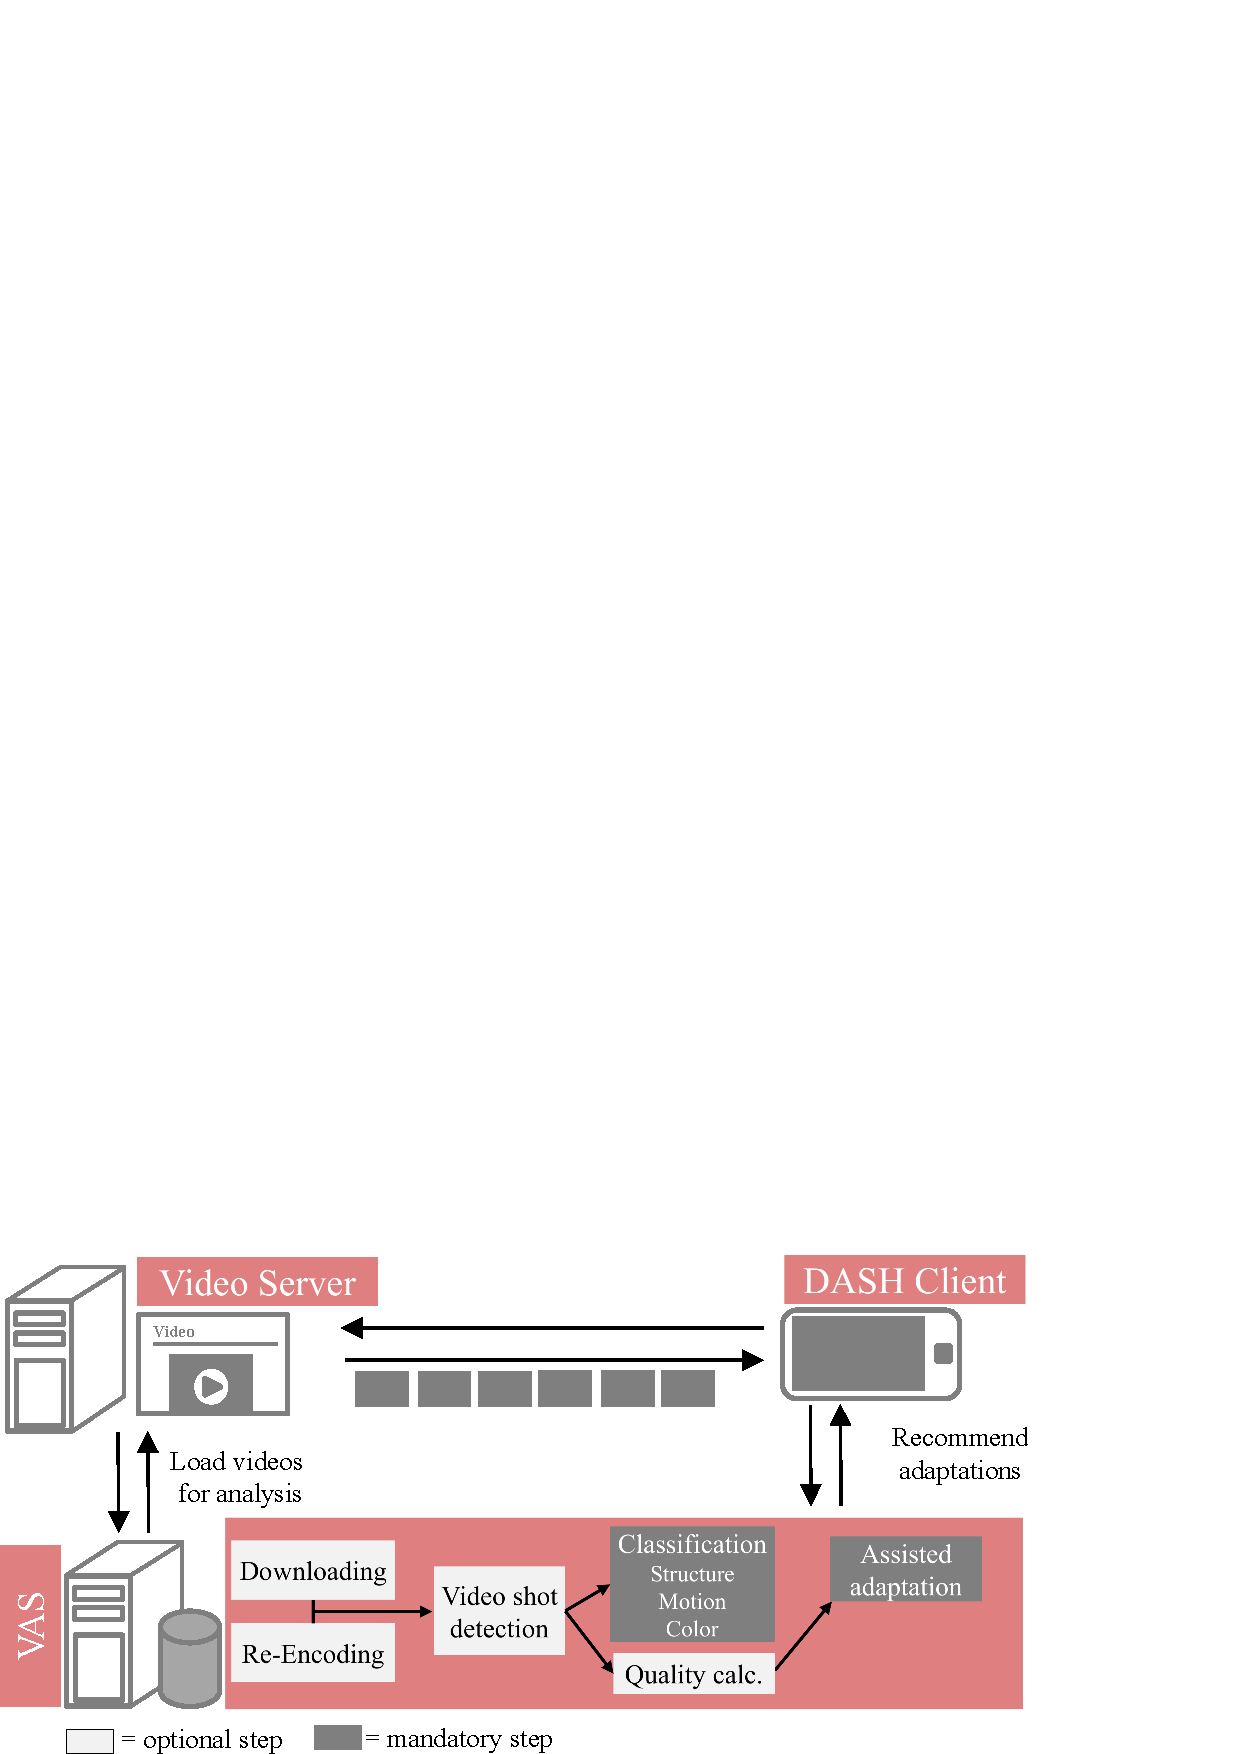
\includegraphics[width=\linewidth]{./gfx/700_VAS/preprocessing.pdf}
	\caption[VAS preprocessing steps]{VAS preprocessing steps are necessary for classifying videos with similar content characteristics.}
	\label{fig:720_preprocessing}
\end{figure}

\ac{VAS} offers adaptations in three quality dimensions of a video: frame rate, 
resolution, and \ac{SNR}, which is solely influenced by the  quantization parameter during the encoding. 
The \ac{SNR} is approximated by the target bit rate of the video, whereas frame rate and resolution are usually described in the \ac{MPD}, an \ac{MPEG} \ac{DASH} manifest. 

The \ac{VAS} analyzes the video which allows for adapting at runtime in a content-aware manner. 
To generate adaptation plans for mobile clients, \ac{VAS} leverages a preprocessing stage that is triggered upon the first request of a video \ac{URL} (see Figure~\ref{fig:720_preprocessing}). 

As content characteristics may change over the course of a video, \ac{VAS} determines chunks in a video stream in which the perceived quality level of a single \ac{MPEG} \ac{DASH} representation is constant.
Figure~\ref{fig:720_preprocessing} illustrates the preprocessing steps described in the following sections.

The depicted preprocessing steps show \ac{VAS}'s answers to the questions of a) What part of the video shall be analyzed? b) How can it be analyzed to quickly determine its perceived quality? and c) How can the process be improved regarding speed? 
\subsubsection{Chunk Preparation}
\label{sec:721_shot_detection}
\ac{VAS} estimates the perceived quality of different representations, but not for an entire video, as it is assumed that quality models may change over time for long-running videos.
A quality model depicts the quality of a video chunk (e.g., regarding the \ac{MOS}) for a given set of \ac{MPEG} \ac{DASH} representations.
Thus, chunks of a video are prepared for which quality models are built.
It was decided that video shots or \ac{MPEG} \ac{DASH} segments are chosen to determine these chunk boundaries.
Whereas the \ac{MPEG} \ac{DASH} segment boundaries are described in the \ac{MPD}, video shots are usually not signaled by streaming services.
If \ac{MPEG} \ac{DASH} segments are chosen as a chunk for quality analysis, no additional preparation step is needed.
Reliably creating quality models for video chunks is difficult for two reasons.
First, perceived quality estimation using objective metrics (such as those proposed in Section~\ref{sec:721_quality_estimation}) usually requires a minimal video duration.
\ac{VQM} requires a duration of more than three seconds which would not allow supporting \ac{MPEG} \ac{DASH} sessions with smaller segments.
The second reason is the assumption that the perceived quality of a video changes with the content.
Another disadvantage of \ac{MPEG} \ac{DASH} segments is the missing ability to map content-characteristic changes.
Figure~\ref{fig:730_QualityVariationSegmentVsShot} compares the estimated quality models based on \ac{MPEG} \ac{DASH} segments with a duration of four seconds and based on video shots.
\ac{MPEG} \ac{DASH} segments as video chunks have the disadvantage that the generated quality models are rather uniform over multiple segments.

In contrast, quality models change significantly over time for video shots.
\begin{figure}[!htb]
	\centering                 
	\subfloat[][]{\includegraphics{./gfx/700_VAS/ploVideoQuality_sID135_step_2}}
	\subfloat[][]{\includegraphics{./gfx/700_VAS/ploVideoQuality_sID104_step_2}}
	\caption[Video quality models generated for video shots and segments]{Comparison of the video quality models evaluated for the video sequence Big Bucks Bunny from the MPEG DASH dataset~\protect\cite{Lederer2012a} using \ac{VQM}. (a) Quality model calculated per four-second \ac{MPEG} DASH segments and (b) Quality model calculated per video shots. Figures show every second representation.}
	\label{fig:730_QualityVariationSegmentVsShot}
\end{figure}
The perceived quality of different encoded representations of an \ac{MPEG} \ac{DASH} video shot is stable, whereas the perceived quality of different shots varies significantly.
This is not a new phenomenon, but is supported for other multimedia applications by Adzic et al. and Akyol et al.~\cite{Adzic2012,Akyol2007}.
The advantage of using video shots is that they quite reliably map content changes with the downside of an additional preprocessing time.
This disadvantage is avoided if the video shots are already known from a composition service such as CrowdCompose or AutoCompose.
If video shot boundary information is not available,
\ac{VAS} uses the edge-change ratio algorithm proposed by Zabih et al.~\cite{zabih1999}.
The algorithm classifies the soon to-be analyzed segments with a hit rate of 86.95\% for hard cuts~\cite{Lienhart1999}. 
In the remaining work, video shots are chosen for our quality models.
\subsubsection{Quality Calculation}
\label{sec:721_quality_estimation}
\ac{VAS} needs to understand the subjective perceived quality of each video representation over time. 
The service leverages an \ac{FR} objective video quality metric, which can decode and analyze different \ac{MPEG} \ac{DASH} representations in parallel and build quality models for video chunks.
An objective \ac{FR} quality algorithm is used to determine the perceived quality of different video representations. 
Besides a reliable prediction of the perceived quality, a short algorithm runtime is favored to support live streaming or video conferencing scenarios. 
None of the existing algorithms combines reliable quality prediction and fast algorithm execution.

The \ac{VQM} algorithm by Pinson et al. is selected to be used in \ac{VAS}~\cite{Pinson2004}.
The essential steps of \ac{VQM} are depicted in Figure~\ref{fig:720_vqmsteps}, and are described in Section~\ref{sec:210_qualitymetrics}.
\begin{figure}[t]
	\centering
	\includegraphics[width=\textwidth]{./gfx/700_VAS/VQMDash}
	\caption[Essential steps of a VQM assessment for \ac{MPEG} DASH videos]{Essential steps of a VQM measurement between a reference representation and other \ac{MPEG} DASH representations (inspired by Pinson et al.~\cite{Pinson2004}).}
	\label{fig:720_vqmsteps}
\end{figure}
In contrast to the discussion in the background chapter, the quality of each \ac{MPEG} \ac{DASH} representation in relation to the highest bit rate representation is assessed.
An algorithm execution starts with a selection of two different \ac{MPEG} \ac{DASH} representations: a reference and a representation to be assessed.
The highest bit rate representation acts as a reference to determine the perceived quality of the lower bit rate representations.
Remaining steps in this approach are similar to the previous discussion.

The quality assessment is repeated for each representation of a video, and quality values are calculated for individual video shots.  
The \ac{VQM} values range from $0$ (no differences between two video sequences to $1$ (significantly impaired video sequence).
For understanding what thresholds classify video into good and bad quality, a mapping is introduced to the well-researched \ac{MOS} concept.
This mapping was studied by Zinner et al.~\cite{Zinner2010}.

The \ac{VQM} implementation is not able to compare reference and test sequences in different resolutions and frame rates internally. 
A real-time quality assessment of \ac{VQM} is developed which allows scaling of videos by leveraging the execution on a \ac{GPU}.
This version is called \ac{RT-VQM}~\cite{Wichtlhuber2016}, but is not part of the discussion in this thesis.
\subsubsection{Classification of Video} 
 As the video quality calculation is computationally intensive, \ac{VAS} classifies the content of a video by visual features and links them to quality models.
Three content characteristics are used for classifying video chunks: colorfulness, structural intensity, and the amount of motion.
 By classifying video chunks, quality models for one video chunk can easily be mapped to any chunk with similar characteristics - even for  different videos.
 A detailed explanation of the contribution of the classification of video chunks is given in Section~\ref{sec:724_videoClassification}.
\subsection{VAS-enabled MPEG DASH Clients}
\label{sec:720_client}
\ac{MPEG} \ac{DASH} clients that want to use \ac{VAS} must allow a minor modification of the video adaptation module.
It is assumed that the \ac{MPEG} \ac{DASH} client stores streamed segments in a playback buffer to compensate for unstable delivery times of video segments.
The filling of the buffer and the adaptation logic of the player are not affected by using \ac{VAS}; however, they can be supported.

Upon starting a streaming session, the client redirects the \ac{MPD} location to the \ac{VAS} server.
This triggers the \ac{VAS} server, which starts evaluation of the video stream to support adaptation. 
The mobile device decides when to consult the service. 
For example, the device contacts \ac{VAS} in cases of throughput fluctuations that force a client to adapt.
In any case, an initialization request is sent to the \ac{VAS} server, triggering the video classification and preprocessing.

For assistance during the streaming session, \ac{MPEG} \ac{DASH} clients regularly request assistance by the \ac{VAS} via a \ac{REST}ful web service.
The web service offers methods (as explained in Section~\ref{sec:721_overview_adaptation_assisstance}) for recommending adaptations to reach the desired quality, and the imperceivable adaptation between representations.
The remote \ac{VAS} server is used for calculating content-aware adaptation plans and returning them to the \ac{MPEG} \ac{DASH} client.
